\documentclass[12pt]{article}
\usepackage[right=1.25in,left=1.25in,top=1.1in,bottom=1.1in]{geometry}
\usepackage{hyperref}
\hypersetup{colorlinks, citecolor=blue, filecolor=blue, linkcolor=blue, urlcolor=blue}
\usepackage{graphicx}
\usepackage{url}
\usepackage[round]{natbib}
\usepackage{amsmath,amsthm} 
\usepackage{engord}
\usepackage{float}
\usepackage{subfig}
\usepackage{pdflscape}
\usepackage{booktabs}
\usepackage{pgfplots}
\pgfplotsset{compat=1.14}
\pgfplotsset{every axis label/.append style={font=\tiny}}
\usepackage[labelsep=period]{caption} %% This switches "Table 1: Title" to "Table 1. Title"

\usepackage{amssymb} %% Necessary, just for the \checkmark command  in tables.
\usepackage{multirow} %% Necessary if we are doing tables in LaTeX
\usepackage{array}
\usepackage{graphicx}
\usepackage{xr}

\usepackage{setspace}
\onehalfspacing

\usepackage{sectsty}
\sectionfont{\large}
\subsectionfont{\normalsize}
\subsubsectionfont{\normalsize}

\newcommand{\specialcell}[2][c]{\begin{tabular}[#1]{@{}l@{}}#2\end{tabular}}

%%%%%%%%%%%%%%%%%%%%%%%%%%%%%%%%%%%%%%%%%%%%%%%%%%%%%%%%%%%%%

\title{ \vspace*{-2.5cm} \hspace*{-0.5cm}Debt Ceiling Brinkmanship and Global Financial Diversification}
% \footnote{
%We are grateful to a first colleague,a second colleague, Tal Gross, No pressure!a fourth colleague, a last colleague,and seminar participants at one university, a second university, and a conferencefor useful feedback. }}

\author{William\thanks{University of British Columbia.
\href{mailto:TK@TK.edu}{wco@student.ubc.ca}}} 
%\and Author Two\thanks{TK University and NBER.  \href{mailto:TK@TK.edu}{TK@TK.edu}} 
%\and Author Three\thanks{TK University. \href{mailto:TK@TK.edu}{TK@TK.edu}}}

\date{ \vspace*{0.5cm} May, 2023\\
%\textbf{Preliminary and Incomplete. \\ Please do not cite or circulate.}
} 

%%%%%%%%%%%%%%%%%%%%%%%%%%%%%%%%%%%%%%%%%%%%%%%%%%%%%%%%%%%%%

\begin{document}

\bgroup
\let\footnoterule\relax

\begin{singlespace}
\maketitle


\begin{abstract}
    \noindent Below is an attached research proposal. It starts with an introduction. Followed by relevant data sets along with proposed methodology. Lastly, a game theory model of debt ceiling brinkmanship is proposed. 
\end{abstract}
\end{singlespace}
\thispagestyle{empty}

\clearpage
\egroup
\setcounter{page}{1}

%% Temporary tool to track how this paper is structured. Feel free to comment in or out. 
% \tableofcontents
% \bigskip

%%%%%%%%%%%%%%%%%%%%%%%%%%%%%%%%%%%%%%%%%%%%%%%%%%%%%%%%%%%%%
%%%%\section{Introduction\label{sec:introduction}}
\section{Introduction 
\label{sec:Introduction}}
We are again experiencing debt ceiling brinkmanship \citep{CFR}. Much work has been done on the possible consequence of not raising the debt ceiling, which would cause havoc on the global economy. Such consequence make it proper to study the debt ceiling. There has also been work on how the debt ceiling brinkmanship momentarily causes market uncertainty, which increases US government borrowing costs, leading to worse fiscal outcomes \citep{Kent_Clark_Center}. We investigate the spillover effects of this mechanism, namely in the context of global financial diversification. A diversified global financial system is optimal in keeping country's incentive aligned such that countries are more likely to cooperate rather than wage war. This leads us to the question.

Does financial diversification increase or decrease given debt ceiling brinkmanship? There can be two results. Parties diversify away from US dollar debt risk. On the other hand, given an global economic uncertainty, parties would pursue the risk free assets, commonly denominated in US dollars. 

\noindent In prior occurrences of government default, like Greece and Argentina, the case to diversify away from such countries was clear and apparent. The US dollar occupies an exorbitant privilege, in that they are the source of the risk at the same time a safe haven. Answering these questions would help us understand weather it would be the world's interest to abolish the debt ceiling system of the united states. 

\section{Dataset 
\label{sec:Dataset}}

We investigate this by using a data set from \citep{Ito_and_Mccauley} on central bank currency composition and official White-house \citep{White_House} data on debt limit raises. Given a raise in the debt limit, we see how central bank's adjust their foreign reserve currency composition. This would be important in assessing how debt ceiling brinkmanship affects foreign central bank diversification. In particular we run regression,
$$\Delta_{UsdShare,t}=\beta_0+\beta_1*\Delta_{Debt Ceiling,t-1}+\sum \beta_i*D_{Countryi,t-1}$$
This would investigate weather the nominal change is a determinant of central bank dollar diversification. 
$$\Delta_{Usd Share,t}=\beta_0+\beta_1*D_{CeilingIncrease,t-1}+\beta_2*D_{CeilingSuspension,t-1}+\sum \beta_i*D_{Countryi,t-1}$$
This would investigate weather the type of brinkmanship is a determinant. 

\noindent Furthermore, we also investigate the spillover effects with respect to other currencies. In other words, how do other currencies get affected from the brinkmanship. If USD is substituted to which currency is it substituted against?\emph{(I am not sure about this equation)}
$$1 = \beta_0+\beta_1*\Delta_{EUR} +\beta_2*\Delta_{JPY}+\beta_3*\Delta_{GBP}+\beta_4*\Delta_{USD}+\beta_4*\Delta_{OtherCurrencies}$$ 

Taking inspiration from this picture.
\begin{figure}[H]
    \begin{center}
    \caption{Another Figure}
    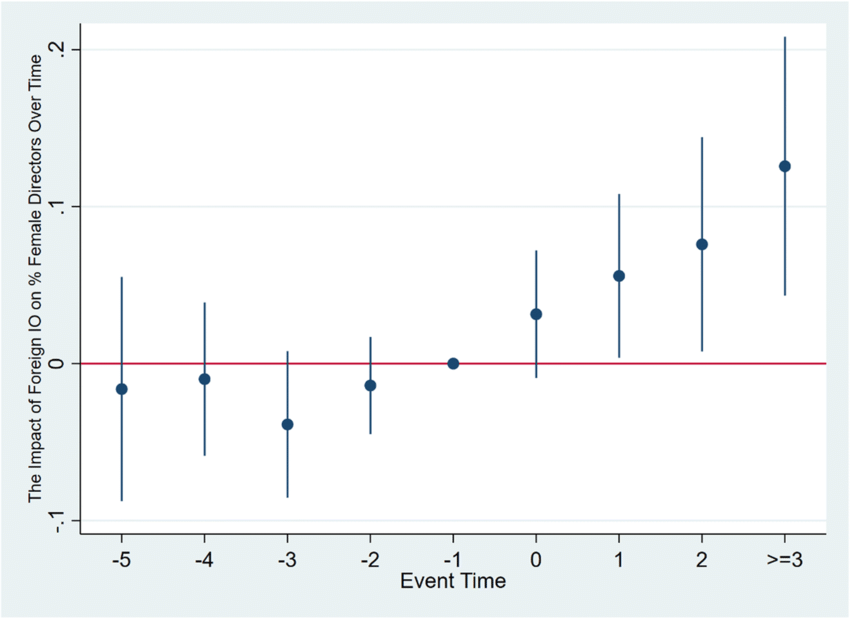
\includegraphics[width=3.0in]{fig/Diagnostic-Test-of-the-Parallel-Trends-Assumption-This-figure-plots-the-coefficients-on.png}
    \end{center}
	\label{fig:mainsummary}
    \vspace{0.2cm}
    \begin{minipage}{0.95\textwidth} 
	{\footnotesize  \ldots
	\par
	}
	\end{minipage}
\end{figure}

\noindent We graph central bank FX reserves with respect to USD, EUR, JPY, GBP, and other currencies. The x axis would be time before and after a debt ceiling increases. The y axis would be the change in composition. 
we run another graph with the x axis reffering the debt ceiling suspensions

$\ast$ 

\noindent We have now investigated our question with respect to central banking. We now investigate aggregate markets. Using external wealth of nations database from Bookings institution \citep{brookings}, we gain access to macro economics financial data, namely 'FX Reserves minus gold to non residents', 'Total liabilities to non residents', 'Portfolio debt liabilities to non residents'. We run regressions.

$$\Delta_{UsTotalLiabilities,t}=\beta_0+\beta_1*D_{Ceiling_Increase,t-1}+\beta_2*D_{Suspension,t-1}$$ Such equation would give us insight into weather foreigners invest into the US, given debt ceiling brinkmanship. 

$$\Delta_{UsPortfolio Debt Liabilities,t}=\beta_0+\beta_1*D_{Ceiling_Increase,t-1}+\beta_2*D_{Suspension,t-1}$$ 
Portfolio debt liabilities would refer to relatively safer liabilities such as bonds. This equation gives us insight into the composition of foreign demand for USD assets. In other words how does brinkmanship affect demand for USD bonds. 

Most importantly we investigate, weather the US central bank itself diversifies its risk. We investigate with regression, 

$$\Delta_{UsFX Reserves,t}=\beta_0+\beta_1*D_{Ceiling_Increase,t-1}+\beta_2*D_{Suspension,t-1}$$

An increase in FX reserves indicates increase in diversification and vice versa. 


We take inspiration from 
\begin{figure}[H]
    \begin{center}
    \caption{Another Figure}
    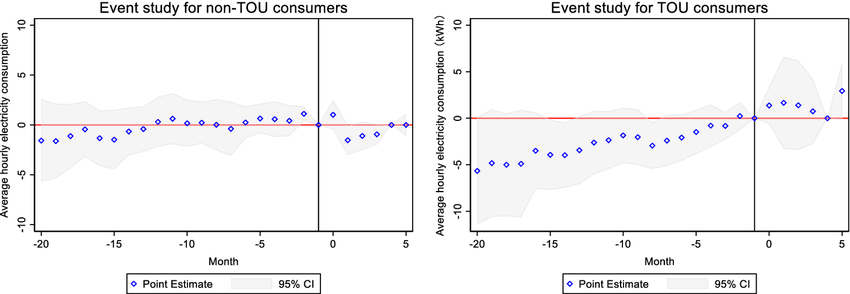
\includegraphics[width=3.0in]{fig/Parallel_Trends_2.png}
    \end{center}
	\label{fig:mainsummary}
    \vspace{0.2cm}
    \begin{minipage}{0.95\textwidth} 
	{\footnotesize  \ldots
	\par
	}
	\end{minipage}
\end{figure}
 \noindent The x axis would mark the dates of debt limit increase and the y axis marks changes in Liabilities to non residents, portfolio debt  liabilities to non residents and US FX reserves. 

\section{Model 
\label{sec:Model}}
We rationalize our finding through a model. We study weather the Debt Ceiling Brinkmanship increases economic welfare.If debt ceiling brinkmanship increases economics welfare then diversification is unnecessary. 


\noindent We first consider a long run model.
Suppose 2 parties $P_l$ and $P_r$, where initally $\pi_l=\pi_r=1/2*Y$. In an ideal world with debt ceiling brinkmanship, for the ceiling to be raised, it must be the case that both parties agree to raise the ceiling such that
$$\pi_l=\pi_r=1/2*Y$$
where $Y$ is GDP. If $\pi_l > \pi_r$, then $P_r$ will not vote to raise the debt ceiling. We assume as an agreement comes to fruition both parties accept condition $\pi_l=\pi_r$. Though the process has a cost, the disagreement raises the cost of capital such that $$\pi_l=\pi_r=1/2*Y-C_d$$
where $C_d$ represents the increase cost of debt.If  $P_l$ and $P_r$ can not come to an agreement then $\pi_{(t),i} = \pi_{(t-1),i}-C_b , \forall i \in \{l,r\}$, where $C_b$ represents the cost of default or "bankruptcy". We assume the initial state wherein $\pi_l=\pi_r=1/2*Y$ such that $\pi_{(t-1),i}=1/2*Y$
$$\pi_{(t),i} = \pi_{(t-1),i}=1/2*Y-C_b , \forall i \in \{l,r\}$$ Now we consider a third party, namely a foreign investor such that 
$(P_L,P_R,Inv)$ would correspond to our payoffs. We let $S$ be the  maximum welfare gain to a foreign investor.
We rationalize this through a game theory table.



\setlength{\extrarowheight}{2pt}
\begin{table}[htbp]
    \resizebox{\textwidth}{!}{
    \begin{tabular}{cc|c|c|}
        & \multicolumn{1}{c}{} & \multicolumn{2}{c}{Party $R$} \\
        & \multicolumn{1}{c}{} & \multicolumn{1}{c}{$Raise$} & \multicolumn{1}{c}{$Not Raise$} \\\cline{3-4}
        \multirow{2}*{Party $L$} & $Raise$ &  $(1/2*Y,1/2*Y,S)$ & $(1/2*Y-C_d,1/2*Y-C_d,S-C_d)$ \\\cline{3-4}
        & $Not Raise$ & $(1/2*Y-C_d,1/2*Y-C_d,S-C_d)$ & $(1/2*Y-C_b,1/2*Y-C_b,S-C_b ) $ \\\cline{3-4}
    \end{tabular}
    }
    \caption{Game Theory Table}
    \label{tab:game_theory}
\end{table} \noindent Intuitively, it must be that $C_b>C_d$. Prior papers have shown that the increased cost of capital from brinkmanship is temporary. But, if a default were to happen this would undoubtedly leave a permanent mark on the US's exhorbitant privilege. With this said, it must be the case that both parties will always Raise such that the equilibirum would be $1/2*Y=\pi_l=\pi_r$. Total welfare being $$W_{with}=Y+S=1/2*Y+1/2*Y+S$$
Next we consider the same scenario without debt ceiling brinkmanship. If so then, $C_d=C_b=0$, which reflects the zero risk of default. We note that $1/2*Y\neq\pi_l\neq\pi_r$. If $\pi_l>\pi_r$ then $C_{ins}>0$ exist, representing the cost of instability such that $$\pi_l=\phi*Y-C_{ins} \pi_r=\eta*Y$$ where $\phi > \eta$ and $\phi+\eta=1$. We then take total welfare such that $$W_{without}=Y-C_{ins}+S=\phi*Y-C_{ins} + \eta*Y+S$$
We conclude $$[W_{with}]>[W_{without}]$$ such that debt ceiling brinkmanship is welfare optimizing. \textbf{This suggest that in the long run, assuming no future shocks occur, diversification is unnecessary.} \\



\noindent $\ast$ We consider the short run wherein $P_i$ will always first proposes $\pi_i=1/2*Y+\epsilon_i$, where $\epsilon_i$ represents some random positive markup. This is the case because $$\mathbb{E}[\pi_i]=\sigma*(1/2*Y+\epsilon_i)+(1-\sigma)*(1/2*Y)$$where $\sigma$ represents the probability of $P_{-i}$ accepting the deal with markup, $\epsilon_i$. We assume $\sigma\approx 0.00001$ such that $$\mathbb{E}[\pi_i]>1/2*Y$$ Likewise, $P_{-i}$ follows a similar strategy. Given this both parties proposals results in $$Y<1/2*Y+\epsilon_r+1/2*Y+\epsilon_d$$This of course is impossible as such parties will always reject in the short run. Following the argument from earlier, if a proposal is rejected the maximum payoff must be$$\pi_{i,pass}=1/2*Y-C_d+\lambda_i , \forall i \in \{l,r\}$$ where $\lambda_i$ represents a positive payoff from party constituents. If both parties reject proposals to default, maximum payoff would be $$\pi_{i,default}=1/2*Y-C_b+\lambda_i, \forall i \in \{l,r\}$$ Because $C_b>C_d$ then $$\pi_{i,pass}>\pi_{i,default} , \forall i \in \{l,r\}$$
Given this both parties will always reject the first proposal but will always accept future proposals. We know consider total welfare. $$W_{with}=Y-2C_d+2\lambda_i+S=2*\pi_{i,pass}+S$$
$$W_{without}=Y-C_{ins}+S$$We know $C_{ins}>C_d$ Furthermore, intuitively $C_{ins}>2*C_d$. Then, suppose $C_{ins}=2*C_d+\theta$ where $\theta$ represents some markup. Then,  $$W_{with}=Y-2C_d+2\lambda_i+S=2*\pi_{i,pass}+S$$
$$ W_{without}=Y-2C_d-\theta+S$$ We know $2* \lambda_i+\theta>0$. Therefore,
$$W_{with}>W_{without}$$ This suggest the debt ceiling brinkmanship is welfare optimal in the short run as well and therefore \textbf{ there should be no financial diversification associated with brinkmanship, in the short run and the long run.} This will be verified with our data sets. 

\section{Literature 
\label{sec:Literature}}
Related work has been done on said topic. Herrera explores US debt ceiling brinkmanship as a stochastic process \citep{Herrera1}. Aye's work not only takes into account debt ceiling, but also governments shutdowns in forecasting US risk premium\citep{Aye}. Another paper from Herrera analyzes brinkmanship from a simpler "do or die" situation\citep{Herrera2}. 










%%%%%%%%%%%%%%%%%%%%%%%%%%%%%%%%%%%%%%%%%%%%%%%%%
\clearpage
\begin{singlespace}
%\bibliographystyle{plainnat}
%\bibliographystyle{chicago}
\bibliographystyle{aer}
\bibliography{our-cites.bib}
\end{singlespace}
%%%%%%%%%%%%%%%%%%%%%%%%%%%%%%%%%%%%%%%%%%%%%%%%%


%%%%%%%%%%%%%%%%%%%%%%%%%%%%%%%%%%%%%%%%%%%%%%%%%
%%%%% These commands start the appendix and change the Table & Figure numbering
\newpage
\appendix
\setcounter{table}{0}
\renewcommand{\tablename}{Appendix Table}
\renewcommand{\figurename}{Appendix Figure}
\renewcommand{\thetable}{A\arabic{table}}
\setcounter{figure}{0}
\renewcommand{\thefigure}{A\arabic{figure}}
%%%%%%%%%%%%%%%%%%%%%%%%%%%%%%%%%%%%%%%%%%%%%%%%%


\end{document}
